\documentclass[11pt]{article}

\usepackage[a4paper,margin=0.75in]{geometry}
\usepackage{amsmath,amssymb}
\usepackage{booktabs}
\usepackage{tabularx}
\usepackage{array}
\usepackage{enumitem}
\usepackage{microtype}
\usepackage{graphicx}
\graphicspath{{docs/}}
\usepackage{float}
\usepackage{placeins}
\usepackage[table]{xcolor}
\usepackage{pgfplots}
\usepgfplotslibrary{groupplots}
\pgfplotsset{compat=1.18}
\usepackage[hidelinks]{hyperref}

\newcolumntype{Y}{>{\raggedright\arraybackslash}X}
\newcommand{\TBD}{\textit{To be completed.}}
\newcommand{\cmark}{\(\checkmark\)}
\newcommand{\pmark}{\(\triangle\)}
\newcommand{\nmark}{--}

\title{Resource-Aware Multi-Agent Reinforcement Learning for Decentralized Maintenance with Shared Heterogeneous Technicians}
\author{Bryan}
\date{Working proposal --- September 2026}

\begin{document}

\maketitle

\begin{abstract}
Decentralized maintenance decisions become coupled when machines share technicians with different service capabilities. A locally attractive maintenance request may increase waiting and cost for other machines. This proposal investigates Resource-Aware QMIX (RA-QMIX), which combines technician-edge utilities, queue-conditioned mixing, and counterfactual consistency in a controlled maintenance simulator with persistent FIFO queues. A five-seed comparison finds the lowest mean objective cost for RA-QMIX among the tested learned methods at the final training budget. A separate ten-seed ablation finds the same final-budget ranking across four evaluation scenarios, although statistically significant superiority is not established in every scenario and fixed policies remain competitive under stress. These results provide initial evidence for the combined architecture. The proposed next steps are to examine the contribution of individual components, validate the modeling assumptions, and assess robustness before extending the system beyond its current fixed size.
\end{abstract}

\section{Background and motivation}

Predictive maintenance is a sequential decision problem under uncertain degradation and failure. A maintenance action can prevent downtime, but it also consumes resources and may be performed before it is economically necessary. In a system with several machines, maintenance decisions are coupled by the availability of technicians.

The coupling has two forms. First, technicians are shared: several machines may request the same technician at the same decision epoch. Second, technicians may be heterogeneous: the service time for a machine depends on the technician selected. Consequently, the best local action for one machine depends on the requests made by the other machines and on the current technician queues.

This proposal studies a decentralized setting in which each machine is a learning agent and technicians are passive resources. The simulator uses a fixed machine-technician service-time matrix to isolate maintenance timing, technician selection, FIFO waiting, and contention. Stage~1 denotes the current fixed-size benchmark and the completed baseline and ablation comparisons. It establishes an initial empirical basis for studying coordination; component attribution, modeling validity, and broader generalization remain open research questions.

\section{Related work and research gap}

The closest prior work is Rodríguez et al.~\cite{rodriguez2022}, which assigns one independent RL agent to each parallel machine and allows an agent to select a technician with technician-dependent repair times. Their conflict semantics treat simultaneous requests for the same technician as invalid actions that incur a penalty and restart the episode. This provides a direct MARL reference, but it does not expose persistent queueing and waiting effects.

Other MARL maintenance studies address maintenance timing, system-level re-optimization, or network decomposition without an explicit heterogeneous technician pool. Shared-resource maintenance studies use restless-bandit or index policies with a centralized controller and generally model repair capacity without identifiable technician skills. Heterogeneous workforce studies model competence, proficiency, routing, and service times, but use MILP, metaheuristics, or a centralized scheduler.

\begin{table}[H]
\centering
\caption{Focused comparison of the most relevant studies.}
\label{tab:related-work}
\scriptsize
\renewcommand{\arraystretch}{1.10}
\setlength{\tabcolsep}{3pt}
\begin{tabularx}{\linewidth}{
    >{\raggedright\arraybackslash}p{2.05cm}
    >{\raggedright\arraybackslash}p{1.90cm}
    >{\raggedright\arraybackslash}p{2.45cm}
    >{\raggedright\arraybackslash}p{3.65cm}
    >{\raggedright\arraybackslash}p{2.75cm}
    >{\raggedright\arraybackslash}X}
\toprule
Study & Agents / decision-maker & Decision scope & Resource and heterogeneity model & Method / comparator & Key distinction from this study \\
\midrule
Rodríguez et al.\\\cite{rodriguez2022} & One RL agent per machine & Timing and technician choice & Shared pool; duplicate requests are invalid and restart the episode; technician-dependent repair times & Independent PPO; corrective, preventive, and random policies & Resolves conflicting requests through penalties and episode restart; this study retains requests in FIFO queues \\
\arrayrulecolor{gray!35}\midrule
Pérez-Hernández et al.\\\cite{perez2024} & MARL agents in localized subnetworks & Local maintenance plans & No explicit technician pool; asset and network heterogeneity & Localized MARL versus network-wide and individual approaches & Organizes maintenance decisions by asset subnetworks rather than by shared technician allocation \\
\midrule
Chen and Liu\\\cite{chen2025} & MARL agents & Replacement timing and inspection interval & No explicit technician resource; RUL and component uncertainty & Sequential multi-objective PPO & Focuses on replacement and inspection decisions rather than technician assignment and queue waiting \\
\midrule
Ruiz-Hernández et al.\\\cite{ruiz2020} & Central controller & Sequential maintenance allocation & Shared repairmen; no technician identity or skill differentiation & Restless-bandit index policy & Uses centralized repair allocation rather than decentralized selection of individual technicians \\
\midrule
Demirci et al.\\\cite{demirci2024} & Central controller & Maintenance under capacity limit & Worker-count capacity; workers are interchangeable & Whittle index and LP lower bound & Represents repair resources as interchangeable capacity rather than individually differentiated technicians \\
\midrule
An et al.\\\cite{an2021} & Central scheduler & Joint production and maintenance scheduling & Shared repairmen with timetables, competence, and availability constraints & HMOBBO with tabu search & Jointly schedules production and maintenance through centralized optimization rather than decentralized policies \\
\midrule
Yu et al.\\\cite{yu2023} & Central scheduler & Task assignment and sequencing & Limited technicians; skills, proficiency, and experience-dependent service times & MILP and modified iterated local search & Optimizes technician task sequences with experience-dependent service times; this study learns machine maintenance requests \\
\midrule
Sanhueza et al.\\\cite{sanhueza2026} & Central planner & Where, when, and by whom to maintain & Multi-base workforce; uni-skilled to multi-skilled technicians; shifts and relocation & MILP and Price-and-Branch & Plans workforce shifts and assignments across bases; this study coordinates requests within a fixed technician pool \\
\arrayrulecolor{black}\midrule
\rowcolor{teal!8}
\textbf{Proposed study} & \textbf{One learning agent per machine} & \textbf{Maintenance timing and technician choice} & \textbf{Fixed shared heterogeneous resources with FIFO queues} & \textbf{RA-QMIX with fixed-policy and value-decomposition baselines} & \textemdash{} \\
\bottomrule
\end{tabularx}
\end{table}
\clearpage

The resulting gap motivates a controlled comparison of decentralized learning methods under heterogeneous technician contention and persistent FIFO queues. Stage~1 isolates this setting so that differences in learning curves, coordination, and objective cost can be assessed under a common simulator and seed protocol.

\section{System architecture}

The proposed system is organized around decentralized machine agents interacting with a shared environment. Each machine agent observes its local condition together with resource-aware technician information, chooses whether to defer maintenance or request a technician, and receives feedback from the resulting assignment and queue dynamics. Technicians are passive resources with fixed skills and service times. RA-QMIX coordinates machine decisions during centralized training and preserves decentralized execution.

\begin{figure}[ht]
\centering
\includegraphics[width=0.98\textwidth]{passive_technician_system_architecture.pdf}
\caption{RA-QMIX system architecture and execution boundary for Stage~1. Machine agents issue decentralized maintenance requests; the environment resolves technician assignment and FIFO queues, while centralized training uses the shared objective.}
\label{fig:system-architecture}
\end{figure}
\FloatBarrier

\section{Research questions and working hypotheses}

\subsection{Main research question}

Can explicitly representing machine--technician compatibility and shared congestion improve decentralized maintenance decisions over standard value decomposition under FIFO queues?

The Stage~1 comparison addresses four experimental questions:

\begin{enumerate}[leftmargin=*]
    \item Does RA-QMIX improve over random feasible and skill-aware FIFO fixed policies?
    \item Does value decomposition improve over independent Q-learning?
    \item Does the resource-aware architecture improve over VDN and standard QMIX?
    \item Do these differences persist across training budgets and the Stage~1 environment cells?
\end{enumerate}

\subsection{Working hypotheses}

\begin{enumerate}[leftmargin=*]
    \item RA-QMIX will achieve lower objective cost than the learned baselines after sufficient training.
    \item Resource-aware utilities, queue-conditioned mixing, and counterfactual consistency will improve coordination under technician contention.
\end{enumerate}

The completed five-seed comparison supports the direction of the first hypothesis on the in-distribution cell. The ten-seed ablation extends the observed final-budget ranking to four scenarios for the tested QMIX variants. The second hypothesis remains only partially assessed: lower objective cost for the combined model does not establish that each component is necessary or that the gain arises from improved coordination. These questions motivate the next experiments.

\section{Problem formulation}

Consider the discrete-time, finite-horizon system implemented by the RL simulator, with machines $i\in\mathcal{M}=\{1,\ldots,N\}$, passive technicians $k\in\mathcal{K}=\{1,\ldots,K\}$, and steps $t=0,\ldots,T-1$. Each machine has an integer operating age $x_{i,t}\in\{0,\ldots,X_{\max}\}$ and a failure indicator $y_{i,t}\in\{0,1\}$. Each technician has a busy-until time $b_{k,t}$, a currently assigned machine $m_{k,t}$ (or $-1$ when idle), and a FIFO queue $q_{k,t}$ of pending machine requests. Each machine appears at most once in the union of all queues and current technician assignments.

The local action of machine $i$ is
\begin{equation}
    a_{i,t}\in\{0,1,\ldots,K\},
\end{equation}
where $a_{i,t}=0$ means defer and $a_{i,t}=k$ means request technician $k$. A fixed service-time matrix $d_{ik}$ represents technician heterogeneity. A lower $d_{ik}$ means that technician $k$ is more capable for machine $i$; an infeasible assignment may be represented by $d_{ik}=+\infty$. A dynamic action mask always leaves defer valid. It masks a nonzero request when the machine is already queued or being serviced, but it does not mask a request merely because the selected technician is busy: such a request is a legitimate FIFO request and may wait in the queue.

The decentralized observation contains the local machine state and public resource features:
\begin{equation}
    o_{i,t}=\left(t,x_{i,t},y_{i,t},
    \{z_{i,k,t}\}_{k\in\mathcal{K}}\right),
\end{equation}
where
\begin{equation}
    z_{i,k,t}=\left(\mathbf{1}[b_{k,t}\leq t],
    \max(0,b_{k,t}-t),
    \mathbf{1}[m_{k,t}=i],
    |q_{k,t}|,
    \operatorname{pos}(i,q_{k,t}),
    d_{ik}\right).
\end{equation}

Thus each technician contributes availability, remaining busy time, self-assignment, queue length, the machine's queue position, and its fixed service time. With $K$ technicians, the observation dimension is $3+6K$. The action mask is part of the environment-policy interface, not an additional learned observation feature.

At each step, all nonzero requests are processed simultaneously. Under the primary FIFO semantics, a request is appended to the selected technician's queue if the machine is not already queued or assigned; every idle technician then pops the oldest queued machine and starts service immediately. Service starts reset that machine's age and failure flag and set the technician's busy-until time to $t+d_{ik}$. Every machine that did not start service ages by one, capped at $X_{\max}$; this includes queued machines. If a nonfailed machine reaches the threshold $A$, it fails with probability $p_{\mathrm{fail}}$ (the current stress cell uses $A=5$ and $p_{\mathrm{fail}}=0.45$). A failed machine remains failed until service starts, and a technician remains unavailable until its busy-until time. The primary semantics use FIFO queues. Priority resolution and the Rodríguez-style invalid-collision rule are retained as diagnostic/ablation semantics. A same-machine duplicate request is rejected and masked; simultaneous requests by different machines for the same technician remain possible and are the intended contention signal.

The finite-horizon objective is to minimize expected cumulative cost:
\begin{equation}
    J(\boldsymbol{\pi}) = \mathbb{E}\left[\sum_{t=0}^{T-1} c(s_t,a_t,s_{t+1})\right],
\end{equation}
where the step cost includes the downtime cost for machines failed at the beginning of the step, maintenance cost for each service that starts, failure cost for newly sampled failures, and queue waiting cost for requests remaining in FIFO queues after service starts. Under the primary FIFO semantics, simultaneous-request collisions are recorded as a diagnostic and do not add a cost; the collision penalty is used only by the priority and invalid-collision ablations. The same transition function, costs, horizon, dynamic action masks, and random-seed protocol will be used for all methods. The learning discount factor is an algorithm hyperparameter and is not part of the environment objective.

\section{Proposed method}

\subsection{Architecture overview}

RA-QMIX adapts monotonic value decomposition to shared heterogeneous technicians through three complementary components. First, a technician-edge utility head scores each machine--technician pairing instead of treating all nonzero maintenance actions as unstructured categories. Second, a queue-conditioned mixer exposes global technician availability and congestion during centralized training. Third, a counterfactual-consistency loss aligns each local action preference with the change in the centralized joint value when only that machine's request changes. The local utilities remain monotonic inputs to the mixer, so execution is decentralized and each machine selects a masked local argmax.

\subsection{Counterfactual consistency}

The counterfactual component is intended to improve credit assignment under resource contention. For example, a machine may choose between joining a busy technician's queue and requesting a slower but available technician. Holding the other machines' actions fixed, the centralized value function estimates the effect of this alternative request on the team. The auxiliary loss encourages the local utility difference to match that estimated joint-value difference. This is a consistency constraint on learned values, rather than a direct observation of the alternative outcome.

Let $Q_i(o_{i,t},a_{i,t})$ be the local utility and let the standard monotonic mixer produce
\begin{equation}
Q_{\mathrm{tot}}(\mathbf{o}_t,\mathbf{a}_t)
=g_\phi\!\left(Q_1,\ldots,Q_N;\,s_t\right),
\end{equation}
where $s_t$ is the concatenation of all local observations used during centralized training. For a valid alternative $a'_{i,t}$, let $\mathbf{a}^{i\leftarrow a'}_t$ replace only machine $i$'s action. The counterfactual loss aligns the local and joint action differences:
\begin{equation}
\mathcal{L}_{\mathrm{cf}}=
\frac{1}{|\mathcal{C}|}\sum_{(i,a')\in\mathcal{C}}
\left[
\bigl(Q_i(o_{i,t},a_{i,t})-Q_i(o_{i,t},a')\bigr)
-\operatorname{sg}\!\left(
Q_{\mathrm{tot}}(\mathbf{o}_t,\mathbf{a}_t)-
Q_{\mathrm{tot}}(\mathbf{o}_t,\mathbf{a}^{i\leftarrow a'}_t)
\right)
\right]^2,
\end{equation}
where $\mathcal{C}$ contains valid alternatives under the current masks and $\operatorname{sg}$ stops the target gradient. Monotonic mixing constrains how the joint value changes with a local utility; the additional loss encourages agreement in the magnitude of the two differences. Whether this regularization improves learning without excessively restricting the value representation remains an empirical question. The training objective is
\begin{equation}
\mathcal{L}=\mathcal{L}_{\mathrm{TD}}+\lambda_{\mathrm{cf}}\mathcal{L}_{\mathrm{cf}},
\qquad
\mathcal{L}_{\mathrm{TD}}=(Q_{\mathrm{tot}}-y_t)^2,
\end{equation}
with
\begin{equation}
y_t=r_t+\gamma(1-d_t)Q^{-}_{\mathrm{tot}}
(\mathbf{o}_{t+1},\mathbf{a}^{\mathrm{greedy}}_{t+1}).
\end{equation}
Here $r_t$ is the negative step cost, $d_t$ indicates episode termination, and the superscript $-$ denotes the target network. The current implementation uses $\lambda_{\mathrm{cf}}=0.05$. The auxiliary term supplies agent-specific supervision during training; execution uses each machine's local observation and public resource information without joint action selection by the mixer.

\subsection{Technician-edge utilities and queue-conditioned mixing}

The technician-edge head separates the defer utility from a score for each technician. With $h_{i,t}=f_\theta(o_{i,t})$, it computes
\begin{equation}
Q_i(o_{i,t},a)=
\begin{cases}
q_i^{\mathrm{def}}(h_{i,t}), & a=0,\\
\langle q_i(h_{i,t}),k_{i,k}(z_{i,k,t})\rangle/\sqrt{d_h}, & a=k.
\end{cases}
\end{equation}
The queue-conditioned mixer appends three summaries per technician to the centralized state: mean availability, maximum remaining busy time, and mean queue length across machine observations. Standard QMIX already receives the underlying resource features through the concatenated observations. The queue extension therefore supplies an explicit representation of congestion rather than additional environmental information. Its intended benefit is to make these features easier for the mixing network to use; the experiments must distinguish this effect from the accompanying change in network capacity.

The full model combines this congestion representation with the technician-edge head and counterfactual loss. The edge head structures local technician scores, the mixer summarizes shared congestion during training, and the loss links local preferences to changes in the learned joint value. Their combined performance and individual contributions are evaluated separately.

\subsection{Comparison algorithms}

Independent Q-learning is the independent value baseline. VDN tests additive value decomposition, while standard QMIX controls for the current RA-QMIX core. Queue-only and counterfactual-only QMIX variants isolate two of its three resource-aware components. Fixed random-feasible and skill-aware FIFO dispatchers provide non-learning references.

\section{Experimental design}

\subsection{Environment cells}

\begin{itemize}[leftmargin=*]
    \item In-distribution cell: three machines and two technicians, horizon $T=12$, failure threshold $A=5$, failure probability $0.45$, and service-time matrix $D=((2,4),(4,2),(3,3))$ under FIFO queues.
    \item Early-failure cell: horizon $18$, failure threshold $4$, failure probability $0.60$, and the base service-time matrix.
    \item Slow-service cell: horizon $18$, base failure parameters, and $D=((3,5),(5,3),(4,4))$.
    \item Combined-pressure cell: the early-failure parameters together with the slow-service matrix.
\end{itemize}

These fixed cells form Stage~1 of the evaluation. The five-seed learning-curve comparison covers the in-distribution cell, while the ten-seed ablation evaluates transfer to the three pressure cells without additional training.

\subsection{Baselines}

Table~\ref{tab:baseline-comparison} summarizes the six primary Stage~1 comparison methods and the two component ablations. The completed comparison uses five training seeds on the in-distribution cell, with common evaluation seeds and fixed checkpoints.

\begin{table}[H]
\centering
\caption{Stage~1 comparison methods and experimental roles. CTDE denotes centralized training with decentralized execution.}
\label{tab:baseline-comparison}
\scriptsize
\renewcommand{\arraystretch}{1.08}
\setlength{\tabcolsep}{3pt}
\begin{tabularx}{\linewidth}{
    >{\raggedright\arraybackslash}p{2.25cm}
    >{\raggedright\arraybackslash}p{1.65cm}
    >{\raggedright\arraybackslash}p{4.25cm}
    >{\raggedright\arraybackslash}X}
\toprule
Method & Class & Experimental role & Evaluation status \\
\midrule
Random feasible & Fixed policy & Non-learning sanity reference; independently samples a valid local action & Stage~1 evaluated \\
Skill-aware FIFO & Fixed dispatcher & Strong resource-aware heuristic using technician availability, FIFO state, and service time & Stage~1 evaluated \\
\midrule
Independent Q-learning & Learned value & Tests learning with independent local utilities and a common team reward & Stage~1 comparison completed \\
VDN & Learned CTDE & Tests whether additive value factorization is sufficient & Stage~1 comparison completed \\
Standard QMIX & Learned CTDE & Primary learned control without dedicated resource-aware modules & Stage~1 comparison completed \\
\midrule
Queue-conditioned QMIX & Ablation & Isolates the effect of explicit queue context in the mixer & Ten-seed ablation completed \\
Counterfactual QMIX & Ablation & Isolates the effect of local--joint difference consistency for credit assignment & Ten-seed ablation completed \\
\rowcolor{teal!8}
\textbf{RA-QMIX} & \textbf{Learned CTDE} & \textbf{Full resource-aware method: edge utilities, queue-conditioned mixing, and counterfactual consistency} & \textbf{Stage~1 comparison completed} \\
\bottomrule
\end{tabularx}
\end{table}

\subsection{Ablation studies}

The ablation study compares four variants to assess the full resource-aware design against standard QMIX and selected individual additions:
\begin{itemize}[leftmargin=*]
    \item \textbf{Standard QMIX:} the baseline without technician-edge utilities, queue-conditioned mixing, or counterfactual consistency.
    \item \textbf{Queue-only QMIX:} standard QMIX with queue-conditioned mixing only.
    \item \textbf{Counterfactual-only QMIX:} standard QMIX with the counterfactual-consistency loss only.
    \item \textbf{RA-QMIX:} the full model combining technician-edge utilities, queue-conditioned mixing, and counterfactual consistency.
\end{itemize}
Comparisons with standard QMIX assess the effect of the selected additions, while comparisons with RA-QMIX test whether the combined design improves on the single-component alternatives. Removing each component from the full model is reserved for future work.

\section{Evaluation protocol and metrics}

Table~\ref{tab:study-overview} summarizes the completed experiments. The primary comparison uses training seeds $11$--$15$ and evaluation seeds $101$--$200$. The ten-seed ablation study uses paired training seeds ($21$--$30$), 100 common evaluation seeds ($1001$--$1100$), and fixed checkpoints at 20,000 and 50,000 episodes. Its policies are trained on the in-distribution cell and evaluated on all four scenarios without adaptation. Section~\ref{sec:ablation-results} reports the ten-seed ablation results.

\begin{table}[H]
\centering
\small
\caption{Roles of the completed experiments. Each trained policy is evaluated on 100 common evaluation seeds within its study; evaluation panels differ between studies. Budgets are training episodes per seed.}
\label{tab:study-overview}
\begin{tabularx}{\linewidth}{@{}p{2.8cm}Ycp{2.3cm}p{2.5cm}@{}}
\toprule
Study & Learned variants & Seeds & Budgets & Evaluation \\
\midrule
Primary comparison & IQL, VDN, QMIX, RA-QMIX & 5 & 5k, 10k, 20k, 50k & In-distribution \\
Ten-seed ablation study & QMIX, queue-only, CF-only, RA-QMIX & 10 & 20k, 50k & All four scenarios \\
\bottomrule
\end{tabularx}
\end{table}

The primary metric is mean total objective cost on common evaluation seeds, with lower values preferred. Secondary diagnostics are:

\begin{itemize}[leftmargin=*]
    \item failure count and downtime;
    \item number of maintenance jobs;
    \item queue waiting and requests to busy technicians;
    \item simultaneous proposal conflicts and invalid duplicate requests;
    \item service-job counts and machine-level service counts when trace instrumentation is enabled;
    \item action diagnostics: unique joint actions, defer fraction, and request count;
    \item robustness across the early-failure, slow-service, and combined-pressure panels.
\end{itemize}

All methods within a scenario use the same failure process, cost coefficients, evaluation seeds, and reporting schema. The independent unit of replication is the training seed; common evaluation seeds estimate each trained policy's conditional mean and are not treated as additional independent replicates. The completed in-distribution comparison records the fixed five-seed protocol and reports mean and across-seed standard deviation at each checkpoint. The ten-seed ablation additionally reports paired mean differences, bootstrap intervals, and Holm-adjusted sign-flip tests. Sealed-test evaluation remains pending.

\section{Completed Stage 1 results}

The completed experiments assess baseline performance and selected component alternatives on the fixed-size benchmark. The two comparisons below use separate training and evaluation seed sets, so their absolute values should be interpreted within each study.

\subsection{Baseline comparison}

The completed comparison uses five training seeds ($11$--$15$), common
evaluation seeds $101$--$200$, and checkpoints at 5,000, 10,000, 20,000, and
50,000 episodes. The fixed policies are evaluated once on the same evaluation
panel; learned policies are evaluated at every checkpoint. Mean objective cost
is reported with the across-training-seed standard deviation for learned
methods, and lower is better.

\begin{table}[H]
\centering
\small
\caption{Completed Stage~1 in-distribution comparison. Values are mean total objective cost with across-training-seed standard deviation in parentheses; fixed policies have no training-seed variation. Lower is better.}
\label{tab:stage1-learning-curves}
\begin{tabular}{lrrrr}
\toprule
Method & 5k & 10k & 20k & 50k \\
\midrule
Random feasible & 61.47 & 61.47 & 61.47 & 61.47 \\
Skill-aware FIFO & 24.84 & 24.84 & 24.84 & 24.84 \\
Independent Q-learning & 103.52 (19.74) & 94.88 (20.73) & 91.70 (24.86) & 11.60 (1.29) \\
VDN & 176.40 (9.83) & 40.00 (21.88) & 20.55 (4.29) & 9.90 (0.65) \\
Standard QMIX & 77.57 (55.44) & 26.94 (7.91) & 21.39 (8.76) & 9.50 (1.17) \\
\textbf{RA-QMIX} & \textbf{40.07 (15.36)} & \textbf{16.10 (8.42)} & \textbf{12.53 (5.55)} & \textbf{8.10 (1.25)} \\
\bottomrule
\end{tabular}
\end{table}

\begin{figure}[H]
\centering
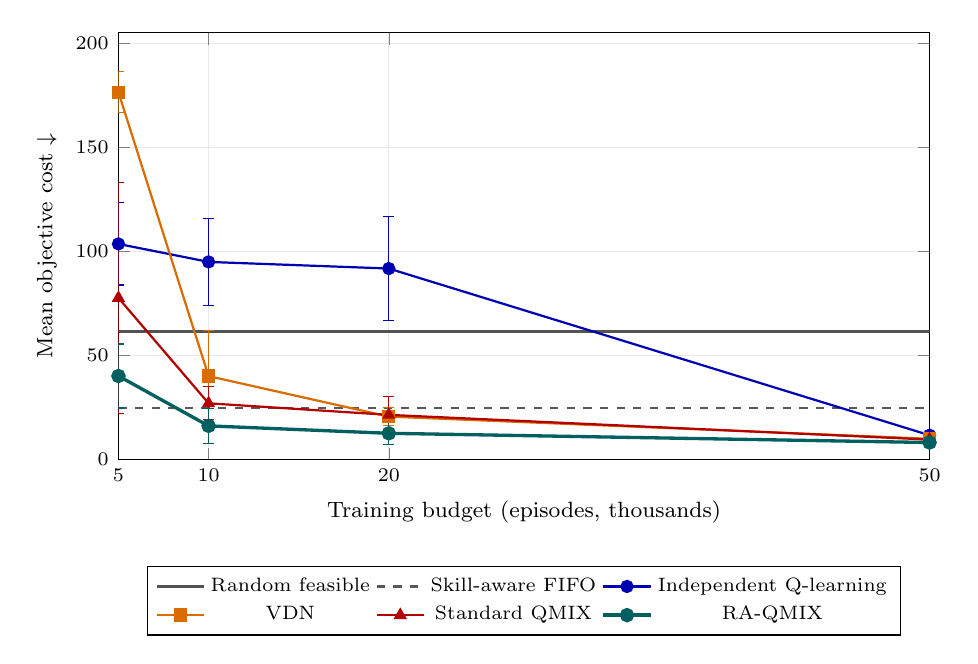
\begin{tikzpicture}
\begin{axis}[
    width=0.98\linewidth,
    height=7.0cm,
    xlabel={Training budget (episodes, thousands)},
    ylabel={Mean objective cost $\downarrow$},
    xmin=5,xmax=50,
    ymin=0,ymax=205,
    xtick={5,10,20,50},
    xmajorgrids=true,
    ymajorgrids=true,
    grid style={gray!18},
    legend style={font=\scriptsize,at={(0.5,-0.25)},anchor=north,legend columns=3},
    tick label style={font=\scriptsize},
    label style={font=\footnotesize},
    error bars/y dir=both,
    error bars/y explicit,
]
\addplot[thick,gray!65!black] coordinates {(5,61.47) (10,61.47) (20,61.47) (50,61.47)};
\addlegendentry{Random feasible}
\addplot[thick,black!65,dashed] coordinates {(5,24.84) (10,24.84) (20,24.84) (50,24.84)};
\addlegendentry{Skill-aware FIFO}
\addplot[thick,blue!70!black,mark=*] coordinates {
    (5,103.52) +- (0,19.74) (10,94.88) +- (0,20.73)
    (20,91.70) +- (0,24.86) (50,11.60) +- (0,1.29)
};
\addlegendentry{Independent Q-learning}
\addplot[thick,orange!85!black,mark=square*] coordinates {
    (5,176.40) +- (0,9.83) (10,40.00) +- (0,21.88)
    (20,20.55) +- (0,4.29) (50,9.90) +- (0,0.65)
};
\addlegendentry{VDN}
\addplot[thick,red!70!black,mark=triangle*] coordinates {
    (5,77.57) +- (0,55.44) (10,26.94) +- (0,7.91)
    (20,21.39) +- (0,8.76) (50,9.50) +- (0,1.17)
};
\addlegendentry{Standard QMIX}
\addplot[very thick,teal!75!black,mark=*] coordinates {
    (5,40.07) +- (0,15.36) (10,16.10) +- (0,8.42)
    (20,12.53) +- (0,5.55) (50,8.10) +- (0,1.25)
};
\addlegendentry{RA-QMIX}
\end{axis}
\end{tikzpicture}
\caption{Stage~1 in-distribution learning curves. Points show the mean objective cost and whiskers show the across-training-seed standard deviation for learned methods; fixed policies are horizontal references. Lower is better.}
\label{fig:stage1-learning-curves}
\end{figure}

At 50,000 episodes, RA-QMIX has the lowest mean objective cost among the
learned methods. Its paired mean differences relative to Independent
Q-learning, VDN, and standard QMIX are $-3.50$, $-1.80$, and $-1.40$,
respectively. Skill-aware FIFO remains a strong fixed reference on this cell.
The ten-seed ablation below extends the evaluation to the three pressure
cells for standard QMIX, queue-only QMIX, counterfactual-only QMIX, and
RA-QMIX.

\begin{itemize}[leftmargin=*]
    \item RA-QMIX is the lowest-cost learned method at all four reported checkpoints on the in-distribution cell.
    \item The 50,000-episode result is a five-seed Stage~1 comparison, not a sealed-test claim.
    \item Fixed policies are reference points rather than training-seed replicates.
\end{itemize}

\subsection{Ablation study}
\label{sec:ablation-results}

The ablation study compares the full RA-QMIX architecture with standard QMIX, queue-only QMIX, and counterfactual-only QMIX over ten paired training seeds. All policies are trained on the in-distribution cell and evaluated on 100 common evaluation seeds in each of four scenarios, without further training on the pressure cells. Standard QMIX provides the baseline without the three resource-aware additions; queue-only and counterfactual-only QMIX each retain one addition, while RA-QMIX combines technician-edge utilities, queue-conditioned mixing, and counterfactual consistency. This comparison tests whether the full design improves on the selected single-component alternatives under both nominal and stressed conditions.

\begin{figure}[!htbp]
\centering
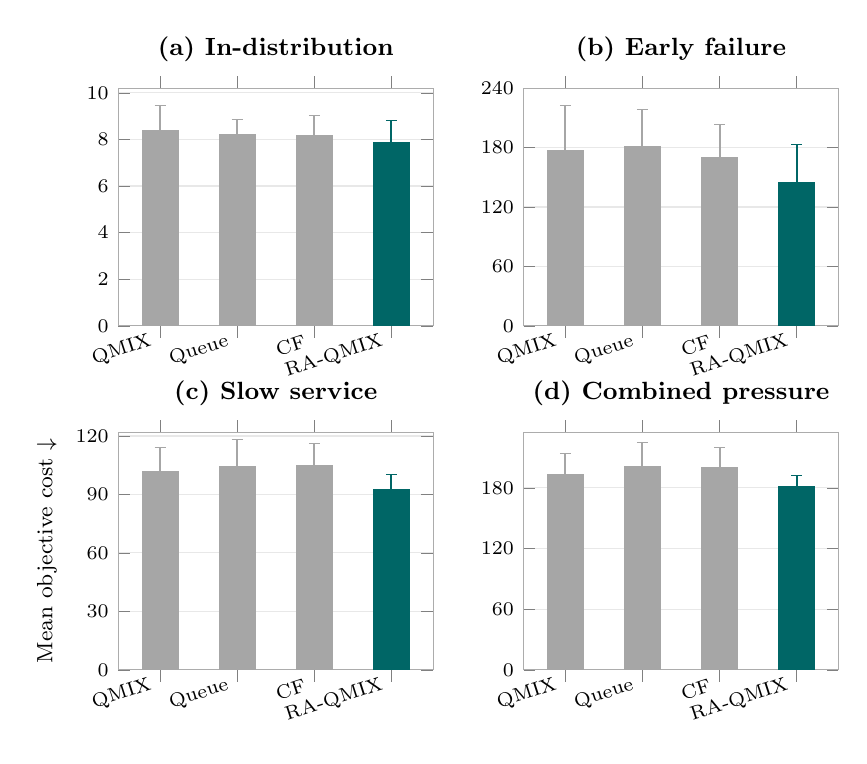
\begin{tikzpicture}
\begin{groupplot}[
    group style={group size=2 by 2, horizontal sep=1.15cm, vertical sep=1.35cm},
    width=0.46\textwidth,
    height=4.6cm,
    ybar,
    /pgf/bar width=13pt,
    every axis plot post/.append style={/pgf/bar shift=0pt},
    enlarge x limits=0.18,
    symbolic x coords={QMIX,Queue,CF,RA-QMIX},
    xtick={QMIX,Queue,CF,RA-QMIX},
    x tick label style={font=\scriptsize,rotate=18,anchor=east},
    ymajorgrids=true,
    grid style={gray!18},
    axis line style={gray!65},
    tick label style={font=\scriptsize},
    label style={font=\footnotesize},
    title style={font=\small\bfseries},
    ymin=0,
    error bars/y dir=both,
    error bars/y explicit,
    error bars/error bar style={line width=0.7pt},
]
\nextgroupplot[title={(a) In-distribution},ymax=10.2,ytick={0,2,4,6,8,10}]
\addplot[fill=gray!48,draw=gray!70,color=gray!70] coordinates {
    (QMIX,8.40) +- (0,1.05) (Queue,8.20) +- (0,0.67) (CF,8.15) +- (0,0.88)
};
\addplot[fill=teal!70!black,draw=teal!80!black,color=teal!80!black] coordinates {(RA-QMIX,7.85) +- (0,0.97)};
\nextgroupplot[title={(b) Early failure},ymax=240,ytick={0,60,120,180,240}]
\addplot[fill=gray!48,draw=gray!70,color=gray!70] coordinates {
    (QMIX,176.60) +- (0,46.25) (Queue,181.41) +- (0,36.64) (CF,170.33) +- (0,33.43)
};
\addplot[fill=teal!70!black,draw=teal!80!black,color=teal!80!black] coordinates {(RA-QMIX,144.94) +- (0,37.76)};
\nextgroupplot[title={(c) Slow service},ymax=122,ytick={0,30,60,90,120},ylabel={Mean objective cost $\downarrow$}]
\addplot[fill=gray!48,draw=gray!70,color=gray!70] coordinates {
    (QMIX,101.69) +- (0,12.62) (Queue,104.40) +- (0,13.71) (CF,104.63) +- (0,11.45)
};
\addplot[fill=teal!70!black,draw=teal!80!black,color=teal!80!black] coordinates {(RA-QMIX,92.69) +- (0,7.77)};
\nextgroupplot[title={(d) Combined pressure},ymax=235,ytick={0,60,120,180,240}]
\addplot[fill=gray!48,draw=gray!70,color=gray!70] coordinates {
    (QMIX,193.23) +- (0,20.26) (Queue,201.09) +- (0,23.44) (CF,200.48) +- (0,19.09)
};
\addplot[fill=teal!70!black,draw=teal!80!black,color=teal!80!black] coordinates {(RA-QMIX,180.99) +- (0,11.44)};
\end{groupplot}
\end{tikzpicture}
\caption{Ablation results at 50,000 training episodes. Bars show the mean of ten training-seed means and whiskers show the across-training-seed standard deviation; lower is better. RA-QMIX is the lowest-cost learned variant in all four reporting scenarios. Queue denotes queue-conditioned QMIX and CF denotes counterfactual-consistency QMIX.}
\label{fig:ten-seed-ablation-results}
\end{figure}

\begin{table}[!htbp]
\centering
\small
\caption{Ablation objective means at 50,000 episodes over ten training seeds. Each training-seed mean uses 100 common evaluation seeds; lower is better. The final column is the paired mean difference relative to standard QMIX.}
\label{tab:ten-seed-ablation-results}
\begin{tabular}{lrrrrr}
\toprule
Scenario & QMIX & Queue & CF & \textbf{RA-QMIX} & $\Delta$ vs. QMIX \\
\midrule
In-distribution & 8.40 & 8.20 & 8.15 & \textbf{7.85} & \textbf{$-0.55$} \\
Early failure & 176.60 & 181.41 & 170.33 & \textbf{144.94} & \textbf{$-31.66$} \\
Slow service & 101.69 & 104.40 & 104.63 & \textbf{92.69} & \textbf{$-9.00$} \\
Combined pressure & 193.23 & 201.09 & 200.48 & \textbf{180.99} & \textbf{$-12.24$} \\
\bottomrule
\end{tabular}
\end{table}

\begin{figure}[!htbp]
\centering
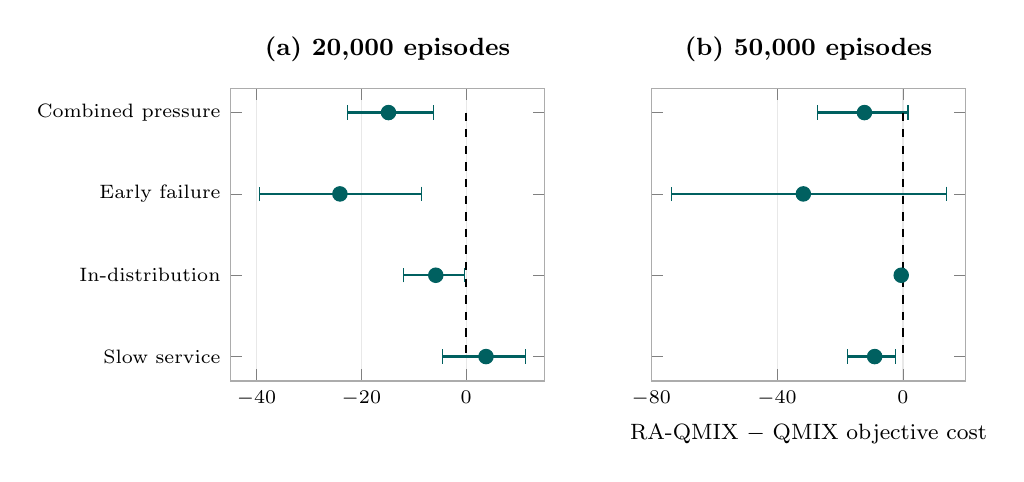
\begin{tikzpicture}
\begin{groupplot}[
    group style={group size=2 by 1, horizontal sep=1.35cm},
    width=0.46\textwidth,
    height=5.3cm,
    symbolic y coords={Combined pressure,Early failure,In-distribution,Slow service},
    ytick=data,
    y dir=reverse,
    xmajorgrids=true,
    grid style={gray!18},
    axis line style={gray!65},
    tick label style={font=\scriptsize},
    label style={font=\footnotesize},
    title style={font=\small\bfseries},
    error bars/x dir=both,
    error bars/x explicit,
]
\nextgroupplot[title={(a) 20,000 episodes},xmin=-45,xmax=15,xtick={-40,-20,0}]
\addplot[only marks,mark=*,mark size=2.6pt,color=teal!75!black,error bars/error bar style={line width=0.8pt}] coordinates {
    (-14.828,Combined pressure) += (8.598,0) -= (7.752,0)
    (-24.089,Early failure) += (15.612,0) -= (15.280,0)
    (-5.814,In-distribution) += (5.487,0) -= (6.115,0)
    (3.764,Slow service) += (7.554,0) -= (8.285,0)
};
\draw[black,dashed,line width=0.6pt] (axis cs:0,Combined pressure) -- (axis cs:0,Slow service);
\nextgroupplot[title={(b) 50,000 episodes},xmin=-80,xmax=20,xtick={-80,-40,0},yticklabels={},xlabel={RA-QMIX $-$ QMIX objective cost}]
\addplot[only marks,mark=*,mark size=2.6pt,color=teal!75!black,error bars/error bar style={line width=0.8pt}] coordinates {
    (-12.238,Combined pressure) += (13.850,0) -= (14.830,0)
    (-31.660,Early failure) += (45.542,0) -= (41.848,0)
    (-0.550,In-distribution) += (1.000,0) -= (1.000,0)
    (-8.996,Slow service) += (6.537,0) -= (8.591,0)
};
\draw[black,dashed,line width=0.6pt] (axis cs:0,Combined pressure) -- (axis cs:0,Slow service);
\end{groupplot}
\end{tikzpicture}
\caption{Paired RA-QMIX effects relative to standard QMIX. Points are paired mean differences across ten training seeds and whiskers are deterministic 95\% bootstrap intervals. Negative values favor RA-QMIX; the dashed line marks no difference.}
\label{fig:paired-effects}
\end{figure}
\FloatBarrier

At 50,000 episodes, RA-QMIX has the lowest mean objective cost among the tested learned variants in all four scenarios (Table~\ref{tab:ten-seed-ablation-results}). Relative to standard QMIX, the reductions are 6.5\% in-distribution, 17.9\% under early failure, 8.8\% under slow service, and 6.3\% under combined pressure. The largest relative improvement occurs under early failure: RA-QMIX also reduces cost from 170.33 for the strongest alternative learned variant, counterfactual-only QMIX, to 144.94. However, both fixed policies remain better than RA-QMIX in this cell, and random-feasible is slightly better under combined pressure. The learned-method ranking therefore does not establish superiority over every maintenance policy.

The effect of training budget depends on the evaluation environment. At 20,000 episodes, RA-QMIX leads the learned variants in three scenarios, while standard QMIX remains best under slow service. From 20k to 50k, RA-QMIX's in-distribution cost decreases from 11.32 to 7.85, but its costs increase from 117.37 to 144.94 under early failure, from 86.13 to 92.69 under slow service, and from 155.92 to 180.99 under combined pressure. All four learned variants show higher mean cost on each pressure cell at 50k than at 20k. Thus, longer training on the nominal cell improves nominal performance without ensuring better transfer. Increased specialization to the training environment is one possible explanation, but the present comparison does not identify the cause.

Paired uncertainty remains substantial (Figure~\ref{fig:paired-effects}). At 50k, RA-QMIX has lower cost than QMIX in 6--8 of the ten paired training seeds, depending on the scenario. The slow-service bootstrap interval excludes zero, while the corresponding Holm-adjusted sign-flip value is $p=0.082$; the other final-budget intervals cross zero. At 20k, the combined-pressure contrast remains significant after Holm correction ($p=0.047$). Correction applies to the three variant-versus-QMIX contrasts within each scenario and budget. These results support the observed mean ranking but do not establish statistically significant superiority across all scenarios.

The ten-seed comparison includes neither edge-only QMIX nor variants that remove one component from the full model. It therefore evaluates the combined architecture against selected alternatives without establishing component necessity or interactions. The sealed test panel remains unevaluated.

\section{Contributions}

The current work provides a controlled formulation of decentralized maintenance with heterogeneous technicians and persistent FIFO queues, together with a resource-aware value-decomposition architecture. The completed comparisons show promising final-budget performance against the tested learned baselines, while revealing uncertainty in component attribution and limitations in transfer to stressed conditions. These are preliminary findings on a small synthetic system.

\section{Scope and limitations}

The completed implementation deliberately treats technicians as passive resources rather than learning agents. It excludes travel and routing, endogenous technician training, outsourcing, and full workforce rostering. Its present evidence comes from a synthetic three-machine/two-technician simulator with a fixed service matrix. The proposal therefore makes claims about Stage~1 coordination and learning curves only.

The completed Stage~1 learning-curve comparison contains five training seeds on the in-distribution cell. A separate ten-seed ablation evaluates four learned variants across four scenarios, but does not include edge-only or leave-one-component-out variants. The sealed final-test panel remains unevaluated. The results should therefore be interpreted as controlled benchmark evidence rather than a deployment guarantee.

\section{Next research steps}

The next stage will test whether the machine--technician relational representation and the auxiliary counterfactual loss improve coordination, or whether the observed gains mainly result from increased network capacity. The planned investigations are:
\begin{enumerate}[leftmargin=*]
    \item \textbf{Component ablation:} remove the technician-edge head, queue-conditioned mixer, and counterfactual loss one at a time from the full RA-QMIX model.
    \item \textbf{Capacity-matched comparison:} compare RA-QMIX with standard QMIX using a comparable number of trainable parameters, under the same observations, training budgets, and evaluation protocol.
    \item \textbf{Loss sensitivity:} vary the counterfactual-loss weight, including zero, to assess its effect on performance and training stability.
    \item \textbf{Coordination analysis:} examine queue waiting, downtime, failures, and maintenance frequency to explain any reduction in total cost.
    \item \textbf{Modeling validation:} compare machine recovery at the start and at the completion of maintenance, and assess how this assumption affects policy behavior and the conclusions.
\end{enumerate}

Future work may extend the evaluation to larger systems and different levels of resource contention by varying the numbers of machines and technicians, their ratio, and the machine--technician service-time matrix.

\begin{thebibliography}{99}

\bibitem{rodriguez2022}
M. L. Ruiz Rodríguez et al., ``Multi-agent deep reinforcement learning based Predictive Maintenance on parallel machines,'' \emph{Robotics and Computer-Integrated Manufacturing}, vol. 78, 102406, 2022. doi: \href{https://doi.org/10.1016/j.rcim.2022.102406}{10.1016/j.rcim.2022.102406}.

\bibitem{perez2024}
M. Pérez-Hernández, A. Puchkova, and A. K. Parlikad, ``Multi-Agent Learning of Asset Maintenance Plans through Localised Subnetworks,'' \emph{Engineering Applications of Artificial Intelligence}, vol. 127, 107362, 2024. doi: \href{https://doi.org/10.1016/j.engappai.2023.107362}{10.1016/j.engappai.2023.107362}.

\bibitem{chen2025}
Chen and Liu, ``Sequential multi-objective multi-agent reinforcement learning approach for system predictive maintenance of turbofan engine,'' \emph{Advanced Engineering Informatics}, 2025. doi: \href{https://doi.org/10.1016/j.aei.2025.103553}{10.1016/j.aei.2025.103553}.

\bibitem{ruiz2020}
D. Ruiz-Hernández, J. M. Pinar-Pérez, and D. Delgado-Gómez, ``Multi-machine preventive maintenance scheduling with imperfect interventions: A restless bandit approach,'' \emph{Computers \& Operations Research}, vol. 119, 104927, 2020. doi: \href{https://doi.org/10.1016/j.cor.2020.104927}{10.1016/j.cor.2020.104927}.

\bibitem{demirci2024}
E. Z. Demirci, J. Arts, and G.-J. van Houtum, ``A restless bandit approach for capacitated condition based maintenance scheduling,'' \emph{Flexible Services and Manufacturing Journal}, vol. 37, pp. 179--207, 2024. doi: \href{https://doi.org/10.1007/s10696-024-09544-y}{10.1007/s10696-024-09544-y}.

\bibitem{an2021}
Y. An et al., ``Flexible job-shop scheduling and heterogeneous repairman assignment with maintenance time window and employee timetable constraints,'' \emph{Expert Systems with Applications}, vol. 186, 115693, 2021. doi: \href{https://doi.org/10.1016/j.eswa.2021.115693}{10.1016/j.eswa.2021.115693}.

\bibitem{yu2023}
X. Yu et al., ``The Field Technician Scheduling Problem with Experience-Dependent Service Times,'' \emph{Mathematics}, vol. 11, no. 21, 4562, 2023. doi: \href{https://doi.org/10.3390/math11214562}{10.3390/math11214562}.

\bibitem{sanhueza2026}
J. I. Sanhueza, F. Delgado, and M. A. Klapp, ``On planning cost-efficient and flexible aircraft maintenance operations: Technician shift scheduling and task assignment over multiple bases,'' \emph{Computers \& Industrial Engineering}, vol. 214, 111801, 2026. doi: \href{https://doi.org/10.1016/j.cie.2026.111801}{10.1016/j.cie.2026.111801}.

\bibitem{schulman2017}
J. Schulman et al., ``Proximal Policy Optimization Algorithms,'' arXiv:1707.06347, 2017.

\bibitem{rashid2018}
T. Rashid et al., ``QMIX: Monotonic Value Function Factorisation for Deep Multi-Agent Reinforcement Learning,'' in \emph{Proceedings of ICML}, 2018.

\end{thebibliography}

\end{document}
